
%% CLASS MANUAL FOUND IN http://blog.poormansmath.net/latex-class-for-lecture-notes/ %%
%% CLASS AUTHOR Stefano Maggiolo %%
\documentclass[english,course]{Notes}

\title{Network \& Operation Systems Essentials}
\subject{Computer Science}
\author{Joao Almeida-Domingues}
\email{2334590D@student.gla.ac.uk}
\speaker{Dr Nikos Ntarmos}
\date{24}{09}{2018}
\dateend{04}{12}{2019}
\place{University of Glasgow}

\graphicspath{{assets/}}

%%%%%%%%%%%% BIB CONFIG %%%%%%%%%%%%%%%
\usepackage[backend=biber, style=reading, citestyle=numeric]{biblatex} 
\usepackage{csquotes}
\newcommand\quo[1]{\begin{displayquote}\ita{\large{#1}}\end{displayquote}}
\bibliography{OOSE} %add bib file name

%%%%%%%%%%% LAYOUT  %%%%%%%%%%%%%%%

\renewcommand{\abstractname}{\vspace{3\baselineskip}} %hack to remove abstract
\usepackage{setspace}
\onehalfspacing

\lstset{
  basicstyle=\ttfamily,
  columns=fullflexible,
  frame=single,
  breaklines=true,
 }
%%%%%%%%%%%%%%%%%%%%%%%%%%%%%%%%

%%%%%%%%%%%%%% KEEP HERE (conflict when in class) %%%%%%%%%%%%%%%%%%%%

 %%%%%MATRICES
    
    \let\mat=\spalignmat
    \let\amat=\spalignaugmat
    \let\vec=\spalignvector
    
%%%%%% row ops
    \newcommand\ro[2]{\xrightarrow[#2]{#1}}
%%%%%%%%%%%%%%%%%%%%%%%%%%%%%%%%%%%%%%%%%%%%%%%%%%%%%

%%%%%%%%%%%%%  PACKAGES (NOT INCLUDED IN CLASS) %%%%%%%%%%%%%%
\usepackage[delims={[]}]{spalign}

%%%%%%%%%%%%%%%% ALGORITHM TEMPLATE %%%%%%%%%%%%%%%%%%%%

%\begin{algorithm}[H]
%\SetAlgoLined\KwData{this text}
%\KwResult{how to write algorithm with \LaTeX2e }initialization\;
%\While{not at end of this document}
%	{read current\;\eIf{understand}{go to next section\;current section becomes this one\;}{go back to the beginning of current section\;}}
%	\caption{How to write algorithms}
%\end{algorithm}

%%%%%%%%%%%%%%%%%%%%%%%%%%%%%%%%%%%%%%%%%%%%%%%%%%%%%

\begin{document}

%%%%%%%%%%%%%%  DISCLAIMER  %%%%%%%%%%%%%%%%%%%%%

\begin{abstract}
	\par{These lecture notes were collated by me from a mixture of sources , the two main sources being the lecture notes provided by the lecturer and the 
content presented in-lecture. All other referenced material (if used) can be found in the \ita{Bibliography} and \ita{References} sections.}
	\par{The primary goal of these notes is to function as a succinct but comprehensive revision aid, hence if you came by them via a search engine , please note 
that they're not intended to be a reflection of the quality of the materials referenced or the content lectured.}
	\par{Lastly, with regards to formatting, the pdf doc was typeset in \LaTeX , using a modified version of Stefano Maggiolo's \href{http://blog.poormansmath.net/
latex-class-for-lecture-notes/}{\underline{\textcolor{blue}{class}}}}
\end{abstract}
\newpage
\newpage

%%%%%%%%%%%%% LECTURES %%%%%%%%%%%%%%%%%%%%%%%

\section{Networks}

\subsection{Introduction - Networked Systems}

	\defn{Networked System}{a collection of autonomous computing devices that exchange data to perform some goal}

	\par{In this first part of the course we'll focus on 3 key aspects of these systems (1) how information is exchanged between the different devices involved ; (2) how we can build larger networks by linking devices ; (3) how systems communicate amongst themselves}

	\defn{Signal}{a function which conveys information}

	\defn{Communication Channel}{component of a a data transfer system responsible for carrying the signal}


	\defn{Information Entrophy}{how much useful information a message is \ita{expected} to contain}

	\par{\ita{Claude Shannon} the father of \ita{Information Theory} showed that the amount of information that can be coded into a message could be quantified, and is known as \ita{Information Enthropy}. Shannon stated that a data transfer system is composed of three parts: a source, a communication channel and a receiver. He identified the main problem within the system was to make sure that the information passed over the channel could be successuflly \ita{recreated} by the source.}

	\par{This encoding and decoding of messages can be done in several ways, some introduce more noise than others, but they all follow the same process of taking some form of physical signal (e.g. a wave) and converting it into some sort of simplied form of itself and then recreating it at the source end}

	\extra{Extra}{Information Enthropy Formal Definition}{
		\par{If we take $X$ as the set of messages $\{x_1 , \dots , x_n\}$ } 
		}

	\defn{Analogue Signal}{a smooth continuum of values}

	\defn{Digital Signal}{a discrete sequence of values}

	\par{The simplest analogue signal is when information is encoded directly using amplitude (e.g. AM radio), however of particular interest to us is the process of converting analogue signals to digital, which can be done for any analogue signal. (see Physical Layer) \rem{the the rate at
	which the signal must be sampled for accurate
	reconstruction is given by the sampling theorem}}

	\subsubsection{Switching}


	\defn{Coding}{the act of mapping information to symbols}

	\defn{Link}{the combination of a signal with a channel}

	\defn{Hosts}{receivers and sources}

	\defn{Network}{a collection of connected links}

	\par{Within a networked system, information flows via channels forming links which connect hosts. The devices connecting the links are called \ita{switches} or \ita{routers} depending on the type of network. This \ita{network switching} is responsible for determining how the information flows through the network and can be setup so that there are dedicated connections between hosts - \ita{circuit switching} - or by splitting the messages into smaller packets before transmission allowing several hosts to share the same channell - \ita{packet switching}}

	\defn{Circuit Switching}{a dedicated circuit between hosts}

	\defn{Packet Switching}{a shared link where messages are split into packets before transmission}

	\par{The main trade-off here is between capacity and availability. For example, traditional phone networks are circuit switched (the very first ones had actual humans switching the channels and connecting hosts) which means that the two hosts requested a channel and they had guaranteed capacity over that channel while the connection was active, but it also meant that if some other hosts needed to use any part of the same link then their connection would be refused.}
	\par{The internet on the other hand, is packet switched, by breaking the messages apart into smalled chunks hosts can share links the catch here being that though connectivity is guaranteed the capacity/speed is dependent on how many users are using the same channel.}



\subsection{Protocols}

	\par{The different building blocks of a network presented above allow for the transportation of information, but is is the use of protocols which provide the semantics. For a message to be decoded the parties involved must agree on some sort of well-defined syntax, so that noise can be separated from meaningul information, this is precisely the role of the various network protocols existing at all levels within a network.}

	\defn{PDU}{stands for protocol data unit, and is the basic unit	of information for any given protocol}

	\par{PDUs can be textual where rules of syntax and grammar are used to implement behaviour (e.g. HTTP), or binary where similar appropriate rules are used (e.g. TCP/IP). It is the role of PDUs to define what messages are legal to send, but is up to protocol semantics to define when to send them and what should be expected in response}

\subsubsection{Layers}

	\par{Communication systems are tipically organised into layers, which reduces complexity at each layer's level. Peers on the same layer, use that layer's protocol to communicate using services provided by the well-defined interfaces of the lower layers}

	\defn{OSI Model}{stands for \ita{Open Systems Interconnection Model} and is a conceptual model that characterises and standardises the communication functions of a telecommunication or computing system without regard to its underlying internal structure and technology. }

	\par{A design tool used widely to model layered communication channels is the \ita{OSI model}. It is merely a design tool, real implementations are more complex and usually the boundaries between layers are not so well defined.}

	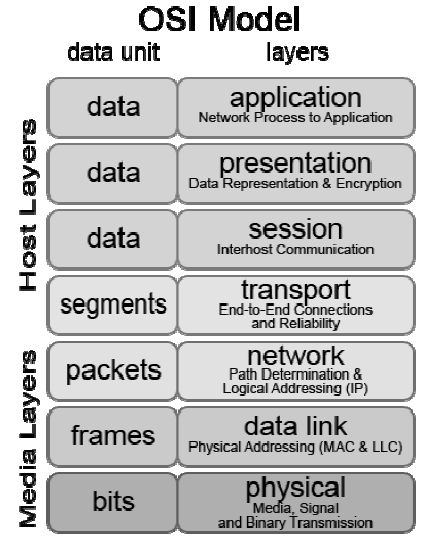
\includegraphics{osi.png}

\subsection{OSI - Physical Layer}

	\par{The physical layer is concernerd with the transmission of raw data bits. In order for this to be possbile, the information needs to be transformed and encoded and a decision on the best medium for the job (e.g. cables, fibre optic etc.) and their phyiscal properties needs to be taken.}

	\subsubsection{Transmission Channels - Enconding \& Modulation}

	\defn{Wired Data Trasmission}{ the signal is transmited over a cable and is \ita{directly} enconded onto the channel, by varying the voltage/light intensity}

	\defn{Wireless Data Transmssion}{ the signal is transmitted without the aid of an electrical conductor, most commonly using radio waves and some kind of modulation}

	\par{A signal can travel with or without the aid of an electrical condutor, if it is directly encoded into a cable, then one of several \ita{enconding schemes} can be used in order to change the signal into discrete pieces of data (e.g. bits).}

		\begin{itemize}
			\setlength\itemsep{0.5em}
			\mymarginpar{High $\approx [3,5]v$ , and Low $\approx [0,3)$}
			\mymarginpar{NRZ : Non-Return to Zero}
			\item\textbf{NRZ : }{1 -- High ; 0 -- Low}
			\item\textbf{NRZ Inverted : }{1 -- Change ; 0 -- Constant}
			\item\textbf{Manchester : }{1 -- High-Low ; 0 -- Low-High}
		\end{itemize}
		

		\todo{Insert image from anki card}

	\par{Alternatively one can encode information onto a channel by varying the properties of the carrier signal via a modulating signal, a process know as \ita{modulation} which allows the same channel to be shared by different signals}

		\todo{Insert image from anki card}

	\subsubsection{Bandwith, Capacity \& Noise}

	\defn{Bandwith}{ determines the frequency range it can transport}

	\defn{Sampling Theorem}{ states that to accurately digitise an analogue signal, $2H$ samples per second are needed, where $H$ is the bandwith in Hz}

	\defn{Signal-to-Noise Ratio}{ the ration between signal power and noise floor, typically quoten in dB $= 10\log(\frac{S}{N})$}

	\par{The bandwidth of a channel is determined by physicial limitations of the channel, and given the existence of noise in the real worl, the \ita{Signal-to-Noise} ratio and the bandwidth represent the fundamental limits for the rate at which information can be transmitted}

	\rem{The maximum transmission rate of a channel grows lograithmically to the SNR}

	\extra{Extra}{Theoretical Maximum Transmission Rate}{

		$$ R_{max} = 2H\log_{2}V $$

		where:
		\begin{itemize}
			\item[]$R_{max} =$ max trasmission rate in bits/s
			\item[]$H =$ bandwith in Hz
			\item[]$V =$ \# of discrete values per symbol
		\end{itemize}
	}

	\extra{Extra}{Shannon's Theorem}{
		$$ R_{max} = H\log_{2}(1 + SNR) $$

	}

	


	
	\subsubsection{Summary}

		\begin{itemize}
			\item\textbf{PDU : } bits
			\item\textbf{Function : } transmit a sequence of bits over an analogue channel
		\end{itemize} 

\subsection{OSI - Physical Layer}

	\par{The physical layer is concernerd with the transmission of raw data bits. In order for this to be possbile, the information needs to be transformed and encoded and a decision on the best medium for the job (e.g. cables, fibre optic etc.) and their phyiscal properties needs to be taken.}

	\subsubsection{Transmission Channels - Enconding \& Modulation}

	\defn{Wired Data Trasmission}{ the signal is transmited over a cable and is \ita{directly} enconded onto the channel, by varying the voltage/light intensity}

	\defn{Wireless Data Transmssion}{ the signal is transmitted without the aid of an electrical conductor, most commonly using radio waves and some kind of modulation}

	\par{A signal can travel with or without the aid of an electrical condutor, if it is directly encoded into a cable, then one of several \ita{enconding schemes} can be used in order to change the signal into discrete pieces of data (e.g. bits).}

		\begin{itemize}
			\setlength\itemsep{0.5em}
			\mymarginpar{High $\approx [3,5]v$ , and Low $\approx [0,3)$}
			\mymarginpar{NRZ : Non-Return to Zero}
			\item\textbf{NRZ : }{1 -- High ; 0 -- Low}
			\item\textbf{NRZ Inverted : }{1 -- Change ; 0 -- Constant}
			\item\textbf{Manchester : }{1 -- High-Low ; 0 -- Low-High}
		\end{itemize}
		

		\todo{Insert image from anki card}

	\par{Alternatively one can encode information onto a channel by varying the properties of the carrier signal via a modulating signal, a process know as \ita{modulation} which allows the same channel to be shared by different signals}

		\todo{Insert image from anki card}

	\subsubsection{Bandwith, Capacity \& Noise}

	\defn{Bandwith}{ determines the frequency range it can transport}

	\defn{Sampling Theorem}{ states that to accurately digitise an analogue signal, $2H$ samples per second are needed, where $H$ is the bandwith in Hz}

	\defn{Signal-to-Noise Ratio}{ the ration between signal power and noise floor, typically quoten in dB $= 10\log(\frac{S}{N})$}

	\par{The bandwidth of a channel is determined by physicial limitations of the channel, and given the existence of noise in the real worl, the \ita{Signal-to-Noise} ratio and the bandwidth represent the fundamental limits for the rate at which information can be transmitted}

	\rem{The maximum transmission rate of a channel grows lograithmically to the SNR}

	\extra{Extra}{Theoretical Maximum Transmission Rate}{

		$$ R_{max} = 2H\log_{2}V $$

		where:
		\begin{itemize}
			\item[]$R_{max} =$ max trasmission rate in bits/s
			\item[]$H =$ bandwith in Hz
			\item[]$V =$ \# of discrete values per symbol
		\end{itemize}
	}

	\extra{Extra}{Shannon's Theorem}{
		$$ R_{max} = H\log_{2}(1 + SNR) $$

	}

	
	\subsubsection{Summary}

		\begin{itemize}
			\item\textbf{PDU : } bits
			\item\textbf{Function : } transmit a sequence of bits over an analogue channel
			\item Information can be encoded directly into the channel or the signal can be modulated
			\item Physicial limitations cap the transfer rate
		\end{itemize} 
\subsection{OSI - Data Link Layer}

	\par{The main purpose of the data link layer is to arbitrate access to the physical layer and turn the raw bit stream of data into a structured communications channel with the goal of transferring data between nodes attached to the same physical cable. There are several services provided by the DDL, the main ones being: \ita{Media Access Control (MAC addressing) , Error detection and/or correction, Framing}}


	\subsubsection{Framing}

		\par{Frames are essentially fenced packets, which signal to the next layer the significant part of the data , i.e the \ita{payload} and often whether that data was corrupted via some sort of error code or \ita{checksum}. The DLL add the final tail and header to the payload and is therefore responsible for the last bit of data \ita{encapsulation}}

		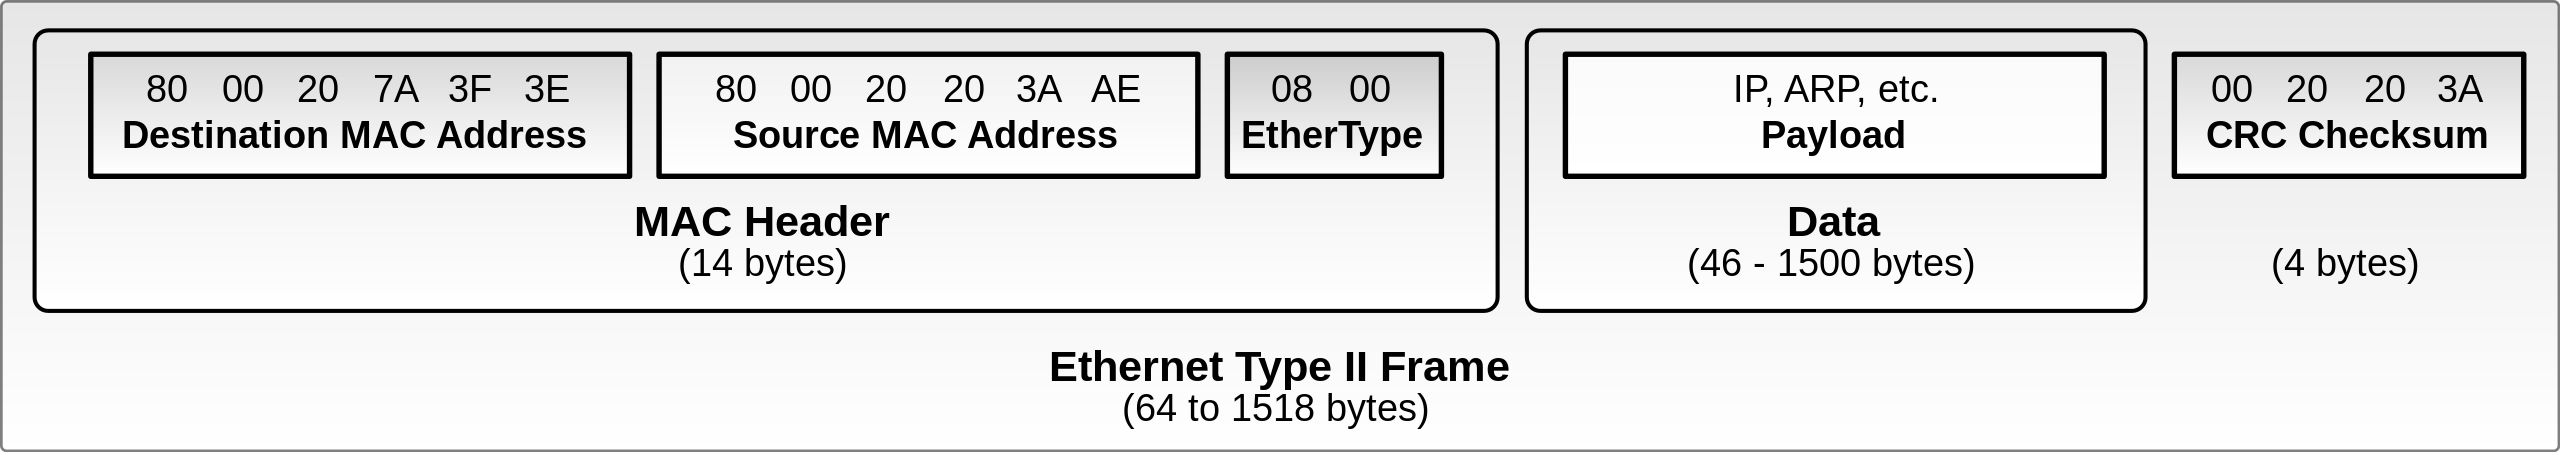
\includegraphics[width=0.7\textwidth]{frame}


	\subsubsection{Error Detection \& Correction}

		\par{Though rare in wired systems, it is quite common for noise to cause bit errors in the data being transmitted. If the DLL implements error detection then it must add a \ita{error detection code} as an header of the frame, the simplest one being the \ita{parity code}. When the receiver gets the packet it uses the same function/rule to recalculate the code, if it doesn't match the frame is either discarded or corrected}

		\defn{Parity Code}{an error detection code which is able to detect single bit errors. It works by adding all the bits, and checking the parity of their sum}

		\defn{Checksum}{works similarly to the parity code, but is able to handle some multiple bit errors by using a 16-bit one's complement checksum}

		\defn{Cyclic Redundancy Code}{a more advanced algorithm, commonly used in the DDL which can check if the bits are out of order. It relies on the remainder of a polynomial division of the data being sent}


	\subsubsection{MAC}

		\par{MAC is needed to determine which machine gets access to the channel when multiple hosts try to access it simultaneously. Because if that happens then the signals are said to \ita{collide} and will overlap, resulting in an unreadable/garbage message.}

		\defn{Contention-Based MAC}{a system is contention-based if multiple hosts share a channel in a way that can lead to collisions}

		\par{CB MAC deals with collision in one of two ways:}

			\begin{enumerate}
				\item \textbf{ALOHA} is the simplest protocol developed at the University of Hawaii in 1970. It tries to transmit whenever data is available, and if a collision occurs the frames are destroyed and the node will wait for a random amount of time before retransmitting, repeating until successful.

				\item \textbf{CSMA} listens to the channel before sending, if it hears no traffic then it starts transmitting. Note however, that if the message takes time to reach the node , i.e. if there's a high \ita{propagation delay} then there is an increased probability of a collision occurring mid-transit, an improved algorithm is \textbf{CSMA/CD} where the sending node keeps listening even during sending, if a collision occurs then both stations cease transmission immediately. This is an improvement because even though the frames are still corrupted, it saves time and bandwidth by reducing the time the channel is blocked due to collision.
				\mymarginpar{The back-of interval between retransmissions is also random, but should increase with the number of collisions to reduce congestion}
			\end{enumerate}

	




	\subsubsection{Summary}
		\begin{itemize}
			\item\textbf{PDU : } series of bits - \ita{frame}
			\item\textbf{Function : } Physical addressing , Framing, Error Detection
			\item Last encapsulation of data step ; adds an error detection code and some other meta data for framing in the trail of the packet
			\item Simpler error detection codes rely on summing up the bits of data and either checking their parity or sum
			\item Contention-Based MAC handle collisions by listening to the channel before sending the data and/or during
		\end{itemize}





%%%%%%%%%%%%% BIB %%%%%%%%%%%%%%%%%%%%%%%

\newpage
\nocite{*}
\printbibliography

\todos

\end{document}